\documentclass{article} % For LaTeX2e
\usepackage{mltemplate,times}
\usepackage{hyperref}
\usepackage{url}
\usepackage{cite}
\usepackage{graphicx}
\usepackage{bm}
\usepackage{amsfonts}
%\documentstyle[nips13submit_09,times,art10]{article} % For LaTeX 2.09






\title{Progress report: A simple PCANet-CNN for Image classification}

\setlength\belowcaptionskip{2pt}

\author{
Yin Zhang \\
Department of Statistics\\
University of Virginia\\
Charlottesville, VA 22903 \\
\texttt{yz4an@virginia.edu} \\
\And
Haoran Liu \\
Department of Computer Science \\
University of Virginia\\
Charlottesville, VA 22903  \\
\texttt{hl4fb@virginia.edu} \\
}

% The \author macro works with any number of authors. There are two commands
% used to separate the names and addresses of multiple authors: \And and \AND.
%
% Using \And between authors leaves it to \LaTeX{} to determine where to break
% the lines. Using \AND forces a linebreak at that point. So, if \LaTeX{}
% puts 3 of 4 authors names on the first line, and the last on the second
% line, try using \AND instead of \And before the third author name.

% newcommand
\newcommand{\fix}{\marginpar{FIX}}
\newcommand{\new}{\marginpar{NEW}}


\nipsfinalcopy % Uncomment for camera-ready version

\begin{document}
\renewcommand{\b}[1] {\boldsymbol{#1}} 
\newcommand{\bb}[1] {\bar{\boldsymbol{#1}}}
\maketitle

\begin{abstract}
%Our proposal is mainly motivated by the PCANet proposed in\cite{chan2015pcanet}, where the PCA filters are learned by extracting the principal components of the image patches. The features learned by PCA filters are on par with, sometimes even better than the most state of the art algorithms. In our proposal, 

In this paper, we are going to propose a simple deep learning architecture for image classification which is based on the PCANet \cite{chan2015pcanet}. In the proposed architecture, we extend the PCANet by connecting it with a convolutional network \cite{krizhevsky2012imagenet}, and the convolutional filters can be learned from back propagation. We will test the proposed deep network in various image datasets for different visual tasks such as CIFAR10 dataset for objection recognition, MNIST dataset for digit recognition and LFW dataset for face verification. We are going to compare the our result with the state of the art and the baselines in \cite{chan2015pcanet}.
\end{abstract}

\section{Motivation and Overview}
This work is mainly motivated by the PCANet, which served as a simple but competitive deep learning baseline. Typically the deep learning networks (DNN) contains stacked trainable stages and is then followed by a supervised loss function. Each stage comprises a fully-connected layer or convolutional layer together followed by a nonlinear neuron function. DNN usually needs time-consuming training via back propagation.

In contrast, PCANet comprises only very basic data processing components. The multi-stage filters are learned by a simple principal component analysis, and no linear operation is involved until its very last layer, where binary hashing and histogram are employed to compute the features. Thus, back propagation is not needed for parameters updating and this results in a very efficient model training. The architecture of PCANet is shown in Figure \ref{Fig1}.

Our goal is to design a novel deep learning architecture, which starts with a PCANet, without binary hashing or histogram, and then is followed by a convolutional network and a supervised loss such as SVM loss or cross entropy loss. Our idea is as follows: the first two stages of PCANet already have learned a very good representation of each image, however, the binary hashing and histogram may lose some information. Therefore, we connect it with convolutional layer(s) and hope the information can be retained as much as possible, thereby leading to a better performance. Since we believe the input features of the convolutional layer(s) are well learned (by PCANet), so we guess it will not take too much time to train the these convolutional filters. 





%\section{Previous work}
%PCANet, CNN

\begin{figure}[h] \label{Fig1}
\vspace{-15pt} \centering
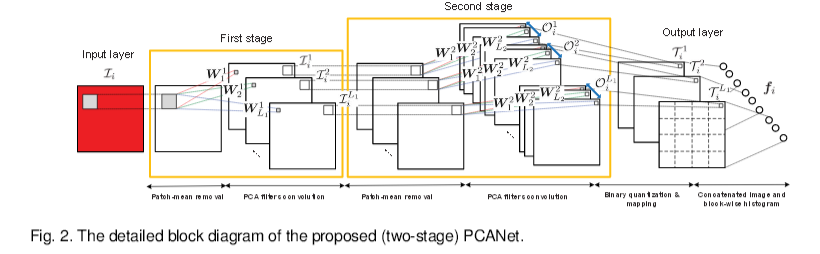
\includegraphics[scale=1.7,width=15cm]{pcanetstructure.png}
\vspace{-20pt}\caption{The Architecture of PCANet}\label{Figure: bspline}
\end{figure}


\section{Model} 
Suppose that we are given $N$ input training images $\{\mathcal{I}_i\}_{i=1}^N $ of size $m \times n$, and assume that the patch size is $k_1 \times k_2$ at all stages in PCANet. The architecture of PCANet is shown in Figure \ref{Fig1}. Here we discard the binary hashing and histogram in the output stage and connect the remaining PCANet with regular convolution layers. The PCA filters only need to be learned from the data one time, but the convolutional filters require to be learned by back propagation. 

\subsection{The first stage of PCA Network (PCANet)}
Around each pixel, we take a $k_1 \times k_2$ patch, and we collect all (overlapping) patches of the $i$th image; i.e., $\b{x}_{i,1},...,\b{x}_{i,mn} \in \mathbb{R}^{k_1\times k_2}$. We then subtract mean from each patch and obtain $\bb{X} = [\bb{x}_{i,1},...,\bb{x}_{i,mn}] $. By constructing the same matrix for all input images and putting them together, we get
\begin{eqnarray}
	\b{X} = [\bb{X}_1,...,\bb{X}_N] \in \mathbb{R}^{k_1k_2\times Nmn}
\end{eqnarray}
In layer $1$, we can obtain the first $L_1$ PCA filters by minimizing the reconstruction error,i.e.
\begin{eqnarray}
	\b{\hat{V}} = \arg\min_{\b{V}\in \mathbb{R}^{k_1K_2\times L_1}} ||\b{X}-\b{VV}^T\b{X}||^2_F  \hspace{0.3cm} \textrm{s.t.} \hspace{0.2cm} \b{V}^T\b{V} = \b{I}
\end{eqnarray}
The solution is known as the $L_1$ principal vectors of $\b{XX}^T$. Then we can obtain the PCA filters by reshaping column $l$ of $\b{\hat{V}}$ to a matrix $\b{W}_l^1$ of dimension $k_1\times k_2$, for $l=1,...,L_1$. The $l$th filter output of the first stage is
\begin{eqnarray}
	\mathcal{I}_i^l =  \mathcal{I} * \b{W}_l^1
\end{eqnarray}
where $*$ denotes the 2D convolution. Therefore, the number of output of first stage is $L_1$, but the size of each output depends on the strides and number of zero paddings.



\subsection{The second stage of PCA Network (PCANet)}
Almost repeating the same process as the first stage. We can collect all the overlapping patches $\mathcal{I}_i^l$ from the first stage, and form $\bb{Y}^l = [\bb{y}_{i,l,1},...,\bb{y}_{i,l,mn}]  \in \mathbb{R}^{k_1K_2\times mn}$, where $\bb{y}_{i,l,j}$ is the $j$th mean-removed patch in $\mathcal{I}_i^l$. We further define $\b{Y}^l = [\bb{Y}_1^l,...,\bb{Y}_N^l]$ for the matrix collecting all the mean-removed patches of the $l$th filter, and concatenate $\b{Y}^l$ for all the filter outputs as 
\begin{eqnarray}
	\b{Y} = [\b{Y}^1,...,\b{Y}^{L_1}] \in \mathbb{R}^{k_1k_2\times L_1Nmn}
\end{eqnarray} 
The PCA filters of second stage are the eigenvectors of matrix $\b{YY}^T$. The number of outputs of the second stage is $L_1L_2$. 

\subsection{Convolutional Network}
We are going to design a 2 layer CNN following the PCANet, and the loss function can be either hinge loss (SVM) or cross entropy loss (logistic regression).

%\section{Experimental design}
\section{Experiments}
We will evaluate the proposed network in various tasks, and compare the results with the state of the art and the baselines in \cite{chan2015pcanet}. At this moment, we just finished the code, and the program is still running. The code is released at \href{https://github.com/tonyzhang1231/PCANet-CNN-torch}{https://github.com/tonyzhang1231/PCANet-CNN-torch}. Unfortunately, we haven't developed the GPU mode for this program, and only CPU mode is available at this moment.

For each task, we plan to set up different cases in terms of varying PCA filter size, number of PCA filters, number of convolutional filters. 

\subsection{Object Recognition on CIFAR10}
\begin{itemize}
	\item Impact of the filter size
	\item Impact of number of PCA filters
	\item Impact of number of convolutional filters
	\item comparison with state of the art
\end{itemize}

\subsection{Digit recognition on MNIST}
\begin{itemize}
	\item Impact of the filter size
	\item Impact of number of PCA filters
	\item Impact of number of convolutional filters
	\item comparison with state of the art
\end{itemize}

\subsection{Face Verification on LFW}
\begin{itemize}
	\item Impact of the filter size
	\item Impact of number of PCA filters
	\item Impact of number of convolutional filters
	\item comparison with state of the art
\end{itemize}


%\subsection{Qualitative evaluation}


%Dataset Details
%\begin{itemize}
%	\item introduction of dataset 
%	\item train size, [val size], test size
%	\item preprocessing details
%\end{itemize}
%
%Framework Details
%\begin{itemize}
%	\item number of layers, the name of each layer, how many filters in each layer
%	\item 
%\end{itemize}
%
%Training Detail
%\begin{itemize}
%	\item how params is initialized
%	\item opt methods, sgd?
%	\item value of learning rate, momentum, batch size, num of epochs, etc
%	\item training time
%	\item a table of training loss, val loss, training accuracy, val accuracy
%\end{itemize}
%
%Evaluation
%\begin{itemize}
%	\item test accuracy
%	\item compare with the state of the art, compare with the result in PCANet.
%\end{itemize}

\section{Future work}
To develop a nn.Module class for PCANet, which inherit the basic nn.Module class. Then it can be integrated into a larger network. The problem we can see so far is that the PCANet can not be placed in the middle of the network. Since if the input of the PCA layers change, we need to retrain the PCA filters, which is super computationally expensive.

\bibliography{mybib}{}
\bibliographystyle{ieeetr}
\end{document}
